\documentclass{article}
\usepackage{packages}
\begin{document}

%\import{./}{title}

\frontmatter
\tableofcontents

\mainmatter
\linenumbers

{\huge{\multiTitle}}

\section*{ABSTRACT}
Key points of article (in no particular order):

\begin{itemize}
    \item warn against the circular reference of assumptions (embedded in data, models, and scenarios); this also includes the points on researcher integrity, transparency, and no-playground.
    \item argue that use of qualifiers (e.g. plausibility) needs to permeate other (secondary) scenario modelling communities.
    \item argue that the criterion of plausibility needs to be time-dependent so that unknown unknowns might be better captured and needs to be applied less strictly (cf. extreme events being not necessarily plausible but important to consider/explore)
    \item models might have to improve to be aligned with basic criteria (e.g. follow thermodynamic laws) such that their underlying functional forms can be compared better (cf. articles by Guivarch (IAMs) and Heijungs (LCA))
    \item argue for better scenario applicability literacy (understand the implications of using specific sets of scenarios (or "scenario ensembles"), i.e. the assumptions embedded in input data, model mechanisms, narratives, and output data), exemplify with SSP marker scenarios. In particular, secondary sustainability scenario modelling should broaden the possibility space. This point also includes that for proper/adequate intercomparison studies, either the applied models or (/and) the underlying calibration + scenario input data must be comparable (in the case of data, they should even be undistinguishable and, if not, complementary); mind, however, that scenario parameters may be determined exogenously for some models while other models may have to be calibrated to those parameters (since they are endogenous variables)...
    \item reflect on reflexivity. Scenarios may inform policymakers and thus influence current course, rendering current scenarios untrue(?; problem of performativity). Relate this point to the no-playground point. (see also \url{https://iopscience.iop.org/article/10.1088/1748-9326/acaf90/pdf}) Also, reflexivity of primary and secondary models: what is primary and what is secondary? Reflexive analysis of secondary or integrated scenarios (as well as of primary scenarios by secondary modellers) via Lazurko's framework is advised.
\end{itemize}

\begin{refsection}

\label{intro}
\section{Introduction}
Socio-ecological systems have long been not accounted for in their full complexity. 
Wicked problems such as climate change gave rise to the field of sustainability science to do so, with prospective analyses having become an important piece in the repertoire \parencite{swart_2004}. 
%The problem of the future is, however, not new, and much can be learnt from other domains of \textit{futures studies}. 
Scenarios can inform the "why", the "what", and, possibly, the "how" of fundamental shifts in interactions in and between socio-ecological systems, something urgently needed (Bentz et al. \url{https://doi.org/10.1007/s11625-022-01123-0}). 
This potential stands up against several challenges to sustainability modelling, such as model validation and the integration of societal dynamics (Elsawah et al. \url{https://sesmo.org/article/view/16226/15789}, McDowall and Geels \url{https://doi.org/10.1016/j.eist.2016.07.001}, Holtz et al. \url{https://doi.org/10.1016/j.eist.2015.05.006})

We want to explore here the emergence of another likely challenge in sustainability scenario modelling: reflexivity and interdependency of assumptions, scenarios, and models across modelling groups and scientific disciplines. 
While reflexivity in sustainability science has been addressed before (Lazurko et al. \url{https://doi.org/10.1016/j.oneear.2023.10.027}), we believe that the role of interaction between quantitative modelling communities has not been made sufficiently explicit. 
In particular, when data (including parameterised scenarios) are generated for and with one (i.e. primary) model and taken up, used, and potentially customised in another (i.e. secondary) model. 
This is of particular importance when reflexive practices are less common in one of the two modelling communities. 

Further, it is our opinion that little attention has been paid to systematic scenario qualification in secondary modelling. 
That is, once (parameterised) scenarios generated with primary models are available, their assumptions, input and output data, as well as implications of their use and integration in secondary modelling are often not critically reflected upon.
Thus, we advocate for more reflexivity of these interactions as well as for performing qualification checks of the adopted and/or customised scenarios. 
In that regard, we devote particular attention to the often-mentioned, yet poorly defined qualifier plausibility, differentiating between its meaning for scenarios and models.

Our paper addresses quantitative sustainability modellers, particularly those working with detailed models in any tradition of sociometabolic research (\url{https://www.nature.com/articles/s41893-019-0225-2}). As there are differences across scientific disciplines and/or across modelling teams in how common scenario modelling is, we first provide some background on sustainability scenario modelling. This includes a run-down of history, an overview of terminology and so-called scenario qualifiers, as well as a review of criticisms voiced against integrated assessment models.
Then, in the main section, we point out how sustainability scenario models may interact iteratively or in parallel and how this can lead to creating a melting pot of assumptions, beliefs, and data.
Lastly, without claiming completeness, we list a range of recommendations to approach this challenge, both for scenario creators and users.


\section{Sustainability scenario modelling}

\subsection{A brief history}
Text from term paper, needs to be drastically shortened.

Scenarios are generally characterised as qualitative or quantitative manifestations of plausible and internally consistent narratives about the future. The antecedents of today's scenario-modelling exercises lie in war games, from where the use of scenarios spread to strategic planning in business and other organisations \parencite{bradfield_2005,schoemaker_1993}.\footnotemark{} With environmental concerns growing during the 1960s-70s, and emphasised by institutions like the Club of Rome and the United Nations, long-term scenario-modelling started to be also used for illuminating potential futures of socio-ecological systems.

A perhaps good resource for background and history on scenario-planning? \url{https://www.tandfonline.com/doi/full/10.1080/00076791.2020.1844667}

\footnotetext{Herman Kahn in the US and Gaston Berger in France were presumably the two most influential figures in these developments.}

Great strides have been made since these pioneering endeavours. And it seems that still more has to be done: While some of the problems addressed by earlier efforts appeared to be only one-dimensional and thus could be dealt with comparatively straightforwardly, we are currently experiencing polycrises in our increasingly volatile, uncertain, complex, and ambiguous world. Some of these crises (individually or combined), may be considered as wicked \parencite{rittel_1973, termeer_2019,lonngren_2021} or even super-wicked problems, such as climate change \parencite{levin_2012}. These are vastly more complex and difficult to solve than other problems that seemed insurmountable at first, such as the ostensible 1894 great horse-manure crisis or the issue of acid rain in late-20$^{th}$ century Europe. These current problems demand therefore more sophisticated approaches, both regarding problem understanding (i.e. modelling) and solving (i.e. policy responses). 

Starting with generic musings by \textcite{daly_1968,isard_1968,cumberland_1966}, \textcite{ayres_kneese_1969} eventually presented in a seminal study how nature-society interactions could be acknowledged more systematically. One can only speculate about their motives of doing so in a neo-classical Walras-Cassel general equilibrium model and not in one more agnostic to economic schools of thought. Yet, before long, interest in this kind of academic exercise spiked rapidly. This was driven by crucial observations like those of Rachel \textcite{carson_1962}, new conjectures on the presumable roots of ecological crises \parencite{white_1967}, and powerful ideas such as the Gaia hypothesis \parencite{lovelock_1972,lovelock_1974}, the concept of a spaceship Earth \parencite{boulding_1966}, and the $I=PAT$ equation \parencite{ehrlich_1972,commoner_1972,chertow_2001}.

Parallel to important contributions in economics on the attribution of current environmental repercussions \parencite[see for example][]{leontief_1970,leontief_1972}, controversial neo-Malthusian concerns à la \textit{Tragedy of the Commons} \parencite{hardin_1968,ostrom_1999,mildenberger_2019} paved the way for the emerging field of world modelling, pioneered by the early activities of the Club of Rome. Different from siloed scientific approaches before, this new field had at its focus the holistic analysis of complex systems such as those which human-nature interactions comprise. Although coarse in detail, initial models like World3 used in \textit{The Limits to Growth} \parencite{meadows_1972} were groundbreaking. Soon after, more refined ones were developed to address the \textit{World Problematique}. The United Nations were instrumental in furthering this work \parencite{fontela_2004}, where some models emphasised the economic aspects (in the tradition of meso-economic and general equilibrium models, e.g. \textcite{leontief_1974}) whereas others focused on interactions within a system of systems (as in systems dynamics, e.g. \textcite{mesarovic_1974}).

With publications such as \textit{Only One Earth} \parencite{ward_1972} and \textit{Our Common Future} \parencite*[WCED,][]{brundtland_1987} documenting the rising necessity to reconsider then-current socio-economic trajectories, the need for quantitative models kept on increasing. Already back then, the important idea of inner and outer limits under various spatio-temporal considerations arose which is popularised today under the name of an inter- and intragenerationally equitable doughnut economy where human needs are satisfied within planetary boundaries; a concept that is in some aspects also approximated by the ideas of deep ecology and strong sustainability. Thus, it is not surprising that the scope of many computational models expanded, both in breadth and in detail. In the following years, various interdisciplinary models (often under the umbrella term of energy-economy models) emerged and first steps in the direction of truly integrated models were undertaken. The meaning of integration goes here in two ways: vertical integration in the sense of linking causes and consequences of environmental issues along their causal chain, and horizontal integration denoting the breadth of causal links as well as cross-topic representations \parencite{parson_1997}. This level of integration has certainly stood in contrast to the granularity of the system representation, and continues to do so today \parencite{krey_2014}.

Hamilton et al. provide another view on integration dimensions \url{https://www.sciencedirect.com/science/article/pii/S1364815214003600}, while Geel et al. caution against expanding unconditional integration \url{https://www.nature.com/articles/nclimate2980}

Although the relevance of a changing climate was acknowledged in the scientific community long before James Hansen's testimony to the US Congress, the first proper integrated assessment model (IAM), RAINS \parencite[developed during the 1980s; for an overview see][]{alcamo_1991}, dealt with acid rain. Yet, RAINS served as a blueprint for similar models that would address climate change and other topics. Such models became relatively quickly part of decision-making processes; as was the case with, for example, ASF \parencite{lashof_1989} and IMAGE \parencite{rotmans_1990} in the first report by the Intergovernmental Panel on Climate Change \parencite*[IPCC,][]{ipcc_1991}.

When speaking of IAMs, one must distinguish between cost-benefit and process-based models: the former are in direct lineage of Coase's concept of social cost and most often are highly aggregated models, whereas most process-based models emerged from the literature on energy modelling and only few were elevated from meso-economic models.\footnotemark{} \textcite{nikas2019,hafner2020} provide useful, detailed classifications of IAMs.

Proctor on heterodox IAMs \url{https://link.springer.com/article/10.1007/s43253-023-00098-7}

A comprehensive comparative evaluation of process-based IAMs is here \url{https://link.springer.com/article/10.1007/s10584-021-03099-9}.

An overview of the IAMs and their historial role at the policy interface \url{https://doi.org/10.1016/j.gloenvcha.2020.102191}

\footnotetext{Cost-benefit models such as PAGE \parencite{yumashev_2019}, FUND \parencite{waldhoff_2014}, and DICE/RICE \parencite{nordhaus_2017} are also termed policy optimisation models, whereas process-based models such as IMAGE \parencite{stehfest_2014}, MESSAGE \parencite{huppmann_2019}, and REMIND \parencite{baumstark_2021} are often referred to as policy evaluation models. The solution concept -- optimisation or simulation -- is, however, not the eponym for these two classes of models; it is rather their use that is the reason for their naming. Cost-benefit models are typically employed to identify the \textit{optimal} balance (based on some criterion) between costs and benefits of policies and impacts. In contrast, process-based models are used to evaluate socio-economic and environmental consequences of actions and impacts; depending on their level of integration and system representation, process-based models are sometimes also referred to as energy-economy-environment (E3) or E4 (E3 + engineering) models. Some models, such as WITCH \parencite{bosetti_2006,emmerling_2016}, can be employed for both policy optimisation and evaluation. In fact, cost-benefit and process-based IAMs may be calibrated to the results of the other \parencite{vanden_2020}, as well as against more complex impact models \parencite{moss_2010}. Both types of IAMs have repeatedly been subject to fundamental criticism \parencite[see for example][]{stern_2016,weyant_2017,keen_2021,gambhir_2019,farmer_2015,pindyck_2017}.}

The spawn of IAMs coincided with sustainability concerns seeping into other scientific disciplines. Earth system models, for example, expanded from modelling only biogeochemical processes of the Earth system to also account for human drivers of changes \parencite{flato_2011}.\footnotemark{} And while it seemed for a while that sociology was slow to pick up on it \parencite{passerini_1998}, it is now rather the case that its potent contribution to sustainability discourses is overlooked \parencite{longo_2021}. Meanwhile, in one branch of engineering, nature-society interactions started to be examined on a rather granular level while still maintaining a system's perspective \parencite{frosch_1989,ausubel_1992}. Characterised by its ideal of cyclic material flows and holistic views \parencite{jelinski_1992}, this new field of industrial ecology thus anticipated the concept of a circular economy \parencite{kalmykova_2018,merli_2018} and, together with other approaches firmly rooted in the respect for thermodynamic principles \parencite{haberl_2019}, the scientific paradigm of socio-economic metabolism \parencite{pauliuk_2015}. An emphasis on thermodynamic principles and roots in physiocratic thinking were also crucial for the emergence of ecological economics, a branch of economics that started growing after, and was moulded by the likes of Robert Ayres, Kenneth Boulding, and Nicholas Georgescu-Roegen \parencite{cleveland_1999}.

\footnotetext{The literature knows many attempts of coupling these models with IAMs. Although primarily \textit{simple} climate and Earth system models such as MAGICC \parencite{meinshauen_2011,meinshausen_2020} have actually been integrated into IAMs \parencite{vanVuuren_2011}, couplings of more complex models have been conducted as well and are expected to become more common \parencite{vanVuuren_2012}.}

Thus, one may observe today a large heterogeneity of models and model families used to analyse socio-ecological systems. These differ not only in their origins and traditions, but also in terms of the aspects they focus on and their underlying principles. For example, IAMs often do not explicitly represent society's biophysical basis, while this is essential to industrial ecology approaches \parencite{pauliuk_2017}. And while industrial ecology and ecological economics share assumptions and considerations, their detail of analysis often differs \parencite{kronenberg_2006}. In addition, one can identify even within model families large differences, such as regarding solution concepts in IAMs or the scale of analysis in industrial ecology.

While some of these differences are not unproblematic, for instance regarding the (dis)respect for thermodynamic laws, one could argue that despite their individual flaws such a large variety of approaches is required to adequately understand socio-ecological systems. Even more so given that in the short time span of the anthropocene \parencite{crutzen_2006}, we have moved quickly from only feeding on nature's free gift \parencite{karsten_1987} to grossly altering our surroundings on all levels in a full world \parencite{daly_2005}. Reports by the IPCC \parencite[e.g.][]{ipcc_2022}, the intergovernmental science-policy platform on biodiversity and ecosystem services \parencite*[e.g. IPBES,][]{ipbes_2019}, and the international resource panel \parencite[e.g.][]{unep_2016} have repeatedly documented humanity's voracity and its consequences. And yet, despite substantially transgressing Earth's biophysical boundaries and getting close to tipping points of all sorts \parencite{ceballos_2015,steffen_2015, steffen_2018}, we are failing on a large scale to achieve social targets \parencite{fanning_2022}.

(An overview of different representations of the future, based on \url{https://www.emerald.com/insight/content/doi/10.1108/FS-01-2021-0020/full/html}
Not sure if it fits here: van Vuuren et al. defined scenario families, categorising earlier global environmental scenario assessments \url{https://www.sciencedirect.com/science/article/pii/S0959378012000635}: economic optimism, reformed markets, global SD, regional competition, regional SD, BAU; newer global scenarios might not fall into any of these categories, as highlighted by Mora et al. for a new set of global land-use + food scenarios \url{https://doi.org/10.1371/journal.pone.0235597})

It is therefore imperative for sustainability science and the associated disciplines to not only understand socio-ecological systems in hindsight \parencite{kates_2001} but also to provide prospective guidance by outlining potential futures \parencite{swart_2004}. This is underlined by both the precautionary principle\footnotemark{} as well as humanity's ancient wish to foresee the future. Although predictions of such complex systems as the human and natural systems are practically impossible, other ways of addressing the future have been devised \parencite{polasky_2011}, with scenario-modelling being well-established in sustainability science. While scenario modelling is the ultimate purpose of IAMs, it has rather slowly been picked up in other domains of sustainability assessment. The IAM community has therefore, and because of their models' comprehensive integration, an advantage as compared to other approaches. Scenario sets originating from the IAM community are highly authoritative and form the basis for global decision-making with regard to climate and other environmental change. Such scenario sets include in particular the representative concentration pathways \parencite[RCPs;][]{vanvuuren_2011_rcp} and the shared socio-economic pathways \parencite[SSPs;][]{riahi_2017,oneill_2014} in the context of climate change. Comprehensive scenario sets for the wider sustainability perspective are less common \parencite{vansoest_2019}, but include notably the sustainable development pathways developed by The World in 2050 initiative \parencite{twi_2018} and those by the SHAPE project \parencite[e.g.][]{soergel_2021}. In addition, modelling approaches from other domains of sustainability science often adopt the assumptions, input parameters, or scenario outputs from these authoritative sources. Examples include the studies by \textcite{deetman_2018,beltran_2020,schandl_2020}. Alternatively, modellers from other fields might devise their own scenarios or rely only partially on larger scenario sets \parencite[for example][]{pauliuk_2013}.

\footnotetext{It should be noted, though, that there are of course different (value-laden) perceptions and definitions of the precautionary principle \parencite{gardiner_2006}. Add \url{https://link.springer.com/article/10.1007/s11406-022-00582-0} and \url{https://www.tandfonline.com/doi/abs/10.1080/10807039991289185} and \url{https://www.tandfonline.com/doi/full/10.1080/21550085.2013.844569}}

Include overview of scenario modelling with LCA, MFA, and IO

\begin{figure} [ht]
    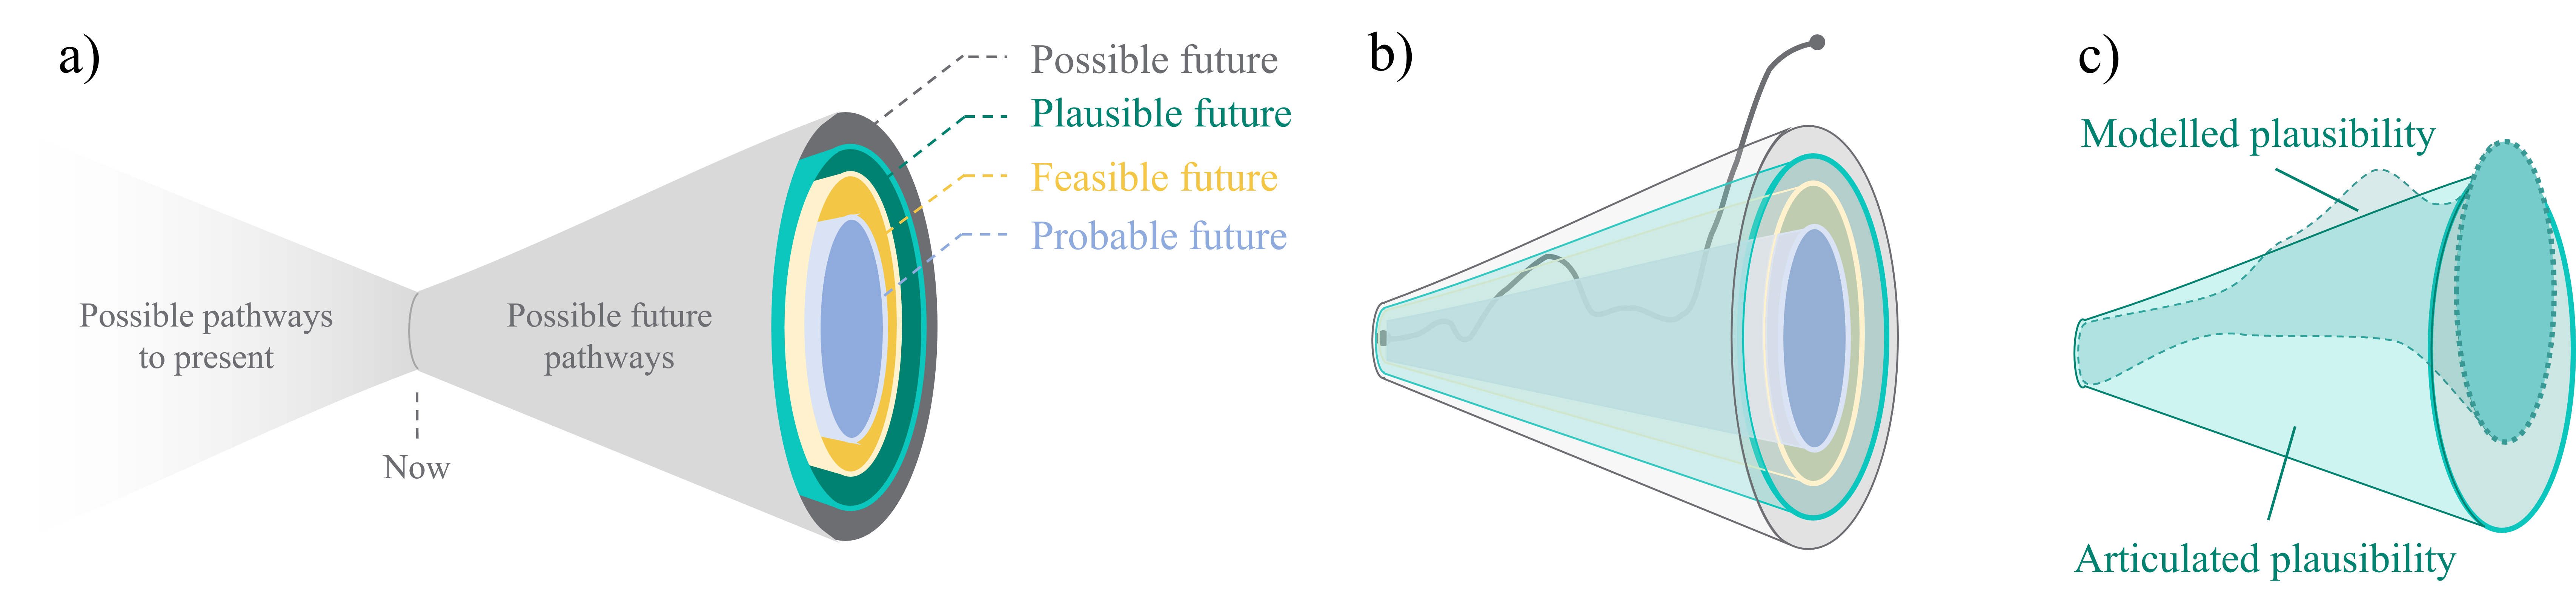
\includegraphics[width=\textwidth]{Cones_plausibility.png} 
    \caption[Some caption for list of figures]{Scenario cones for a variable of interest. a) Multiple alternative futures are possible, which may be narrowed down through the use of qualifiers. b) Extreme events may lie outside of what we currently consider possible. c) Scenarios depend on models and (explicit or implicit) storylines (=ideas of the future), both of which may be qualified in terms of their plausibility, which is not necessarily congruent. 
    Source: 1.a) Adapted from Jewell and Cherp \url{https://wires.onlinelibrary.wiley.com/doi/10.1002/wcc.838}, 1.b) adapted from McCollum et al. \url{https://www.nature.com/articles/s41560-020-0555-3}, 1.c) own elaboration.}  
    \label{fig:plausibility}
\end{figure}


\subsection{The scenario process}

Spaniol and Rowland on defining "scenario" \url{https://onlinelibrary.wiley.com/doi/10.1002/ffo2.3} and a response by Chermack \url{https://onlinelibrary.wiley.com/doi/full/10.1002/ffo2.13}, supporting many points made but also objecting others, e.g. that scenarios need narratives.

Elsawah et al. on the scenario process \url{https://www.sciencedirect.com/science/article/pii/S0048969720319069}

Distinguish scenarios from counterfactuals as Booth et al. do \url{http://dx.doi.org/10.1016/j.futures.2008.07.037}. Both are types of modal narratives, but while scenarios are future-oriented, counterfactuals refer to the past (with what-if questions)

Various scenario typologies exist, a popular one being the one by Börjeson et al. Bishop et al. on scenario typologies and similar \url{https://www.emerald.com/insight/content/doi/10.1108/14636680710727516/full/pdf?title=the-current-state-of-scenario-development-an-overview-of-techniques}. Other typologies and classifications are provided/summarised by Amer et al. \url{https://www.sciencedirect.com/science/article/pii/S0016328712001978}, or earlier by van Notten et al. \url{https://www.sciencedirect.com/science/article/pii/S0016328702000903}

Related to that, have a look at the scenario intervention typology by Crawford \url{https://www.sciencedirect.com/science/article/pii/S0040162519306924?via%3Dihub}


\subsubsection{Scenario elements}
Assumptions, beliefs, ideas, emotions, values, norms...

Observations, expectations, imaginaries, narratives \url{https://journals.sagepub.com/doi/full/10.1177/00380385221138010#fn2-00380385221138010}

Scenario inputs (data, models, narratives etc) and outputs, processes, and objectives \url{https://www.annualreviews.org/doi/full/10.1146/annurev-environ-112321-095011}


\subsubsection{A jungle of scenario qualifiers}
Possibility, probability, likeliness, plausibility, feasibility, desirability, consistency, contingency.

Uruena as prime source on meaning and role of plausibility \url{https://www.sciencedirect.com/science/article/pii/S0016328718303264?via%3Dihub} Fischer and Dannenberg might continue along these lines \url{https://www.sciencedirect.com/science/article/pii/S0016328721000380?via%3Dihub} and Glette-Iversen in the risk context \url{https://www.sciencedirect.com/science/article/pii/S0925753521004756?via%3Dihub}

Ramirez and Selin on the distinction between plausibility and probability \url{https://www.emerald.com/insight/content/doi/10.1108/FS-08-2012-0061/full/html}. (Interestingly, they actually question the depiction of the future as a cone... maybe I should mention in the figure caption that the shape was arbitrarily chosen to be conic but that in reality it may take any shape)

Wiek et al. are an important references as well \url{https://www.researchgate.net/profile/Lauren-Keeler/publication/263276841_Plausibility_indications_in_future_scenarios/links/573b616508ae9ace840ea713/Plausibility-indications-in-future-scenarios.pdf}

Futures pyramid by Dorsser et al. \url{https://www.sciencedirect.com/science/article/pii/S0016328717302513?via%3Dihub}

Walton et al. on "theory of plausibility" with case study in New Zealand \url{https://www.sciencedirect.com/science/article/pii/S0016328718300892?via%3Dihub#bib0375}

Schmidt-Scheele discusses how users of scenarios assess their plausibility \url{https://www.sciencedirect.com/science/article/pii/S2211467X20301243?via%3Dihub#bib24}

Fischer and Dannenberg on plausibility, emphasising many of Uruena's points \url{https://doi.org/10.1016/j.futures.2021.102729}

Janasik again on plausibility vs probability \url{https://www.sciencedirect.com/science/article/pii/S0016328720301609?via%3Dihub}

Plausibility in IAMs via fiction, by van Beek and Versteeg \url{https://www.sciencedirect.com/science/article/pii/S001632872300099X?via%3Dihub}

In 2.2.8, van Vuuren et al. refer to scenario classifiers (=qualifiers?): saliency, credibility, legitimacy \url{https://www.sciencedirect.com/science/article/pii/S0959378012000635}

Walton et al. developing a theory of plausibility in scenario building \url{https://doi.org/10.1016/j.futures.2019.03.002}

Vervoort et al. might provide some good recap of existing divide regarding probability (positivist camp) and plausibility (constructivist camp (post-normal?)) \url{https://www.sciencedirect.com/science/article/pii/S0016328715001184}

Another view on plausibility by Hajer and Pelzer? \url{https://www.sciencedirect.com/science/article/pii/S2214629618300732}

Robertson on transparency in IPCC modelling \url{https://wires.onlinelibrary.wiley.com/doi/full/10.1002/wcc.679}

Braunreiter et al. argue that scenarios should support rather than narrow down deliberations on possible and desirable futures \url{https://www.sciencedirect.com/science/article/pii/S2214629621003133}

Schmidt-Scheele on plausible energy scenarios \url{https://www.sciencedirect.com/science/article/pii/S2211467X20301243}

Jewell and Cherp on feasibility spaces \url{https://wires.onlinelibrary.wiley.com/doi/10.1002/wcc.838}

\subsubsection{Limiting criteria}
Explain why plausibility is a better criterion than the too-vast possibility and the conditional (because based on past and present trends into the unknown future) probability

Plausibility as an epistemic device, scenarios as perception devices (uruena). He also argues that plausibility requires an additional identifier/criterion.

Plausibility used in the scenario creation process and as a criterion for evaluating a scenario. (Uruena describes this as methodological-delimiting and anticipatory-enabling.) I guess one might add that plausibility could also be added as a criterion in the model generation process (if validation is not or only at high costs possible)
Moreover, in terms of using plausiblity as a criterion for evaluating scenarios, it is important to consider that very heterogenous user groups may use the constructed scenarios, but were maybe not involved in the scenario construction process. These users might therefore be confronted with a large number of different and potentially contradicting scenarios such that they have to evaluate their plausibility differently (+ by different means) from how users would who were engaged in the construction process. See book by Schmidt-Scheele \url{https://www.degruyter.com/document/doi/10.1515/9783839453193/html?lang=en}. In that book, the author also shows that users rate scenarios' plausibility according to source credibility, i.e. who constructed the scenarios, and according to how likely the scenarios appears to be, i.e. it is based on individual beliefs and expectations...

At the same time, plausibility is subjective. Would pre-cautionary approaches admonish us to think BIG and thus consider rather possibility?
At the same time, some have argued that applying precautionary approaches requires the identification of plausible threats...
Tipping points are of course of more uncertain nature, but other climate impacts and other environmental impacts more generally are more certain


\subsection{Sustainability scenario models}
Overview of IAMs

Overview of other models (SMR)

Distinguish between consequential and attributional models (employ terms from LCA); call them alternatively impact/state/causal and imputation models.

As for IAMs (text from term paper; needs to be drastically shortened):

Today's sustainability scenario-modelling is largely dominated by the IAM community, their models, and the scenarios that they develop. While the development process for the most authoritative global change scenarios has evolved from moving only sequentially along the causal chain to a more parsimonious, parallel process \parencite{moss_2010} and ultimately combining scenario sets in a matrix architecture \parencite{vanvuuren_2014},\footnotemark{} SSPs rely just like RCPs (and often other frameworks, too) on marker scenarios. That is, for each of a set of agreed upon narratives there is one representative scenario implementation chosen. Non-marker scenarios can then be understood as alternative scenario interpretations \parencite{riahi_2017}. The marker scenarios are, however, the authoritative ones and are exclusively implementations made with major IAMs such as AIM \parencite{fujimori_2017}, GCAM \parencite{calvin_2017}, and MESSAGE \parencite{fricko_20171}. When such scenarios are then taken over by other assessment methods, it is usually only the marker scenarios that are employed, thus introducing a bias towards the bigger IAMs (and thus towards large modelling teams that might also receive comparatively more funding). Also across different scenario sets, there is a bias towards larger IAMs: among all 1,686 vetted pathways explored in the IPCC Sixth Assessment Report database using a pool of more than 20 models, about one third was computed using MESSAGE and REMIND \parencite{gambhir_2022,byers_2022}.

\footnotetext{Although many goals were achieved with this scenario architecture, the common sentiment among respective modellers is that further improvements must be made, such as the integration of societal conditions \parencite{oneill_2020}. Others have raised their voices concerning the plausibility of some scenario combinations, such as SSP3-RCP7.0 or RCP5-SSP8.5 \parencite{pielke_2022}.}

Differentiate between scenario adaptation and/or customisation and ignorant use of numbers. This review could be useful \url{https://www.annualreviews.org/doi/full/10.1146/annurev-environ-102017-030109}

On the other hand, these major IAMs have some of the most comprehensive socio-ecological system representations available. Other scenario-modelling approaches that focus only on a subsystem (e.g. a sector, or in terms of a partial equilibrium) might yield inconsistent modelling outcomes and scenario sets. The reason for this is simply that feedback effects (including rebound effects) might not be accounted for, thus potentially resulting in inconsistent dynamics of the system. In addition, insights from such exercises may be hard to compare to the outcomes from more comprehensive (although perhaps coarser) assessments.

Among IAMs, there are great differences in terms of model structures, input assumptions, and model outcomes \parencite{krey_2014,krey_2019,hiroto_2020,keppo_2021}. It may thus happen that one ends up comparing apples and oranges. For example, when a model (say, one relying on intertemporal optimisation) is fundamentally different from another one (e.g. a myopic systems dynamics model), and when their data parameterisations of the same aspects differ, too, one cannot expect to obtain like interpretations for a common exercise.\footnotemark{} Although the issue has already been recognised \parencite{giarola_2021}, there may continue to be cases where modelling outcomes are more sensitive to the choice of IAM than to the input parameterisation \parencite{sognnaes_2021}. At the same time, the case of similar models yielding different results because of only different parameterisations is hardly surprising either. On an even more fundamental level, IAMs might diverge in their worldviews, with many among the cost-optimizing frameworks following neoclassical assumptions. Well-known problematic aspects following from these worldviews often include the application of discount rates \parencite{emmerling_2019}, non-coverage  of capital trade (because of the otherwise occurring Lucas paradox \parencite{lucas_1990,keppo_2021}), a disregard for emerging behaviours \parencite{farmer_2015}, or unrealistic behavioural assumptions \parencite{asefi_2021}. Another issue is certainly when input or output parameters from one model (which might be based on neoclassical assumptions) are uncritically adopted by other modelling efforts that might have entirely different (and thus inconsistent) assumptions (e.g. post-Keynesian) - or where even the parameter sets are contradictory for some variables. It is even more problematic when results from these secondary efforts might find their way back again into the first set of models, thus creating a wild mix in terms of assumptions and parameterisations.\footnotemark{}

% Similar to Sognnaes et al., some studies pointed out "that the differences between the models [IAMs and global land use models] analyses were greater than the differences between different scenarios modelled" \url{https://www.sciencedirect.com/science/article/pii/S1877343518301362} in intro. Along similar lines, the very same article cites a study that pointed out that most global land use models have never been validated \url{https://esd.copernicus.org/articles/8/369/2017/} (haven't read it yet)

\footnotetext{On that note, it need be mentioned that the selective use of some scenarios and their (mis)interpretation is a topic in itself which has been addressed multiple times already \parencite{pielke_2021}, e.g. regarding the use of RCP8.5 as a baseline scenario \parencite{hausfather_2020}.}

\footnotetext{Importantly, some of the input assumptions of IAMs may be too coarse to use as an input for more disaggregated secondary modelling. It should be noted, however, that there also exist multi-sectoral IAMs of higher resolution; they do rely on different assumptions and principles, though \parencite{lefevre_2022}.}

A recent article by Pereira on challenges of (IAM-based) top-down scenarios \url{https://www.tandfonline.com/doi/full/10.1080/26395916.2021.1901783}, including complexity, uncertainty, cross-scale evaluation, participation etc.

These and other issues are the reasons for why it has been argued that IAMs do not explore the full possibility space \parencite{keppo_2021,mccollum_2020, gambhir_2022}. Assumptions integral to individual models then become inevitably implicit in scenario sets developed with these models. Since explicit and implicit value choices are made in the construction of both the IAMs and their scenario sets (and the underlying narratives, respectively), care must be applied when interpreting the outcomes of such efforts \parencite[even if it is only reference scenarios; see e.g.][]{grant_2020} - and even more so when adopting them for further (secondary) analysis with models from other domains. Given the relevance of global change scenarios for policy-making, one moves thus quickly from questions of intrinsic to extrinsic ethics, meaning that the wider society might be affected by modellers' judgements \parencite{beck_2016},\footnotemark{} for instance in terms of implicit justice perceptions \parencite{rubiano_2022}. One might even go so far as to allege a bias towards Western value sets, given that most of the IAMs are being developed in respective countries which are then also predominantly employed in multi-model comparison studies \parencite{duan_2019}.

\footnotetext{Given that wicked problems such as those addressed with IAMs cannot be "tamed" with only a reductionist approach \parencite[nor is it morally justifiable to do so;][]{churchman_1967}, especially not under the precautionary principle, ethical values come inevitably into play when widening the analysis' subject and the respective comprehensive modelling. This is typically the case when social dynamics are part of the problem -- as is common for wicked problems.}

As of now, IAMs are our best shot to tackle large-scale (or even wicked) problems comprehensively, but they fail on different levels. Especially the incomplete (and sometimes inadequate; cf. neoclassical assumptions) coverage of socio-economic dimensions in these models creates a bias towards irrational (although some economists might call it rational for exactly that) futures. Such model assumptions and biases are perpetuated and disseminated through respective scenarios to secondary modelling efforts and to the wider discourse on topics of global change. It is therefore that we argue that we need to move beyond these conventional scenario-modelling efforts and towards \textit{real} ones.

Then on extremes.
\textcite{mccollum_2020} argue that IAMs should more vehemently explore extreme scenarios so as to account for transient (i.e. low-probability) events (e.g. sudden and widespread recessions), disruptive drivers (e.g. disintegration of political alliances), and unexpected outcomes (e.g. technological change). \textcite{gambhir_2022} point out that current IAMs do not allow for such a more complete exhaustion of the possibility space. 

On IAM scenario ensembles \url{https://www.nature.com/articles/s41558-022-01349-x}

For more trans-/interdisciplinary modelling, focusing on circular economy \url{https://doi.org/10.1016/j.spc.2021.12.011}

Regardless of choosing matrix, morphological, or other scenario architectures, a translation step from qualitative to quantitative is necessary. Doing this transparently is important for credibility, reusability, reproducibility etc. A review on this step for land use has been conducted by Mallampalli et al. \url{https://www.sciencedirect.com/science/article/pii/S1364815216301037}. They review various methods applicable for that, including expert interviews, ABM, fuzzy cognitive maps, causal loop diagrams...

\subsection{Possibility, solution, and target spaces: where is the future?}

Define possibility space, solution space, and target space.

Also mention "scenario space" as Braunreiter et al did (\url{https://doi.org/10.1016/j.erss.2021.102220})

On target space (of SDGs) \url{https://www.cell.com/one-earth/pdf/S2590-3322(22)00003-3}

Keppo et al. on exploring the possibility space; basically a review of and response to criticisms towards IAMs (\url{https://iopscience.iop.org/article/10.1088/1748-9326/abe5d8})

Scenarios are more than continuations of past legacy.

Future path dependency depends on past, present, and future decisions. Future path dependency does not continue right from present path dependency - the time in between matters and may feature creative and other disruptions. Therefore, plausibility is time-contingent.

Talk about black swans as well as grey swans / dragon kings and grey rhinos. 
(And with that also talk about regime changes, (social + natural) tipping points etc.)
An evaluation of alleged black swan events \url{https://www.sciencedirect.com/science/article/pii/S0013935120300190}


\begin{figure} [ht]
    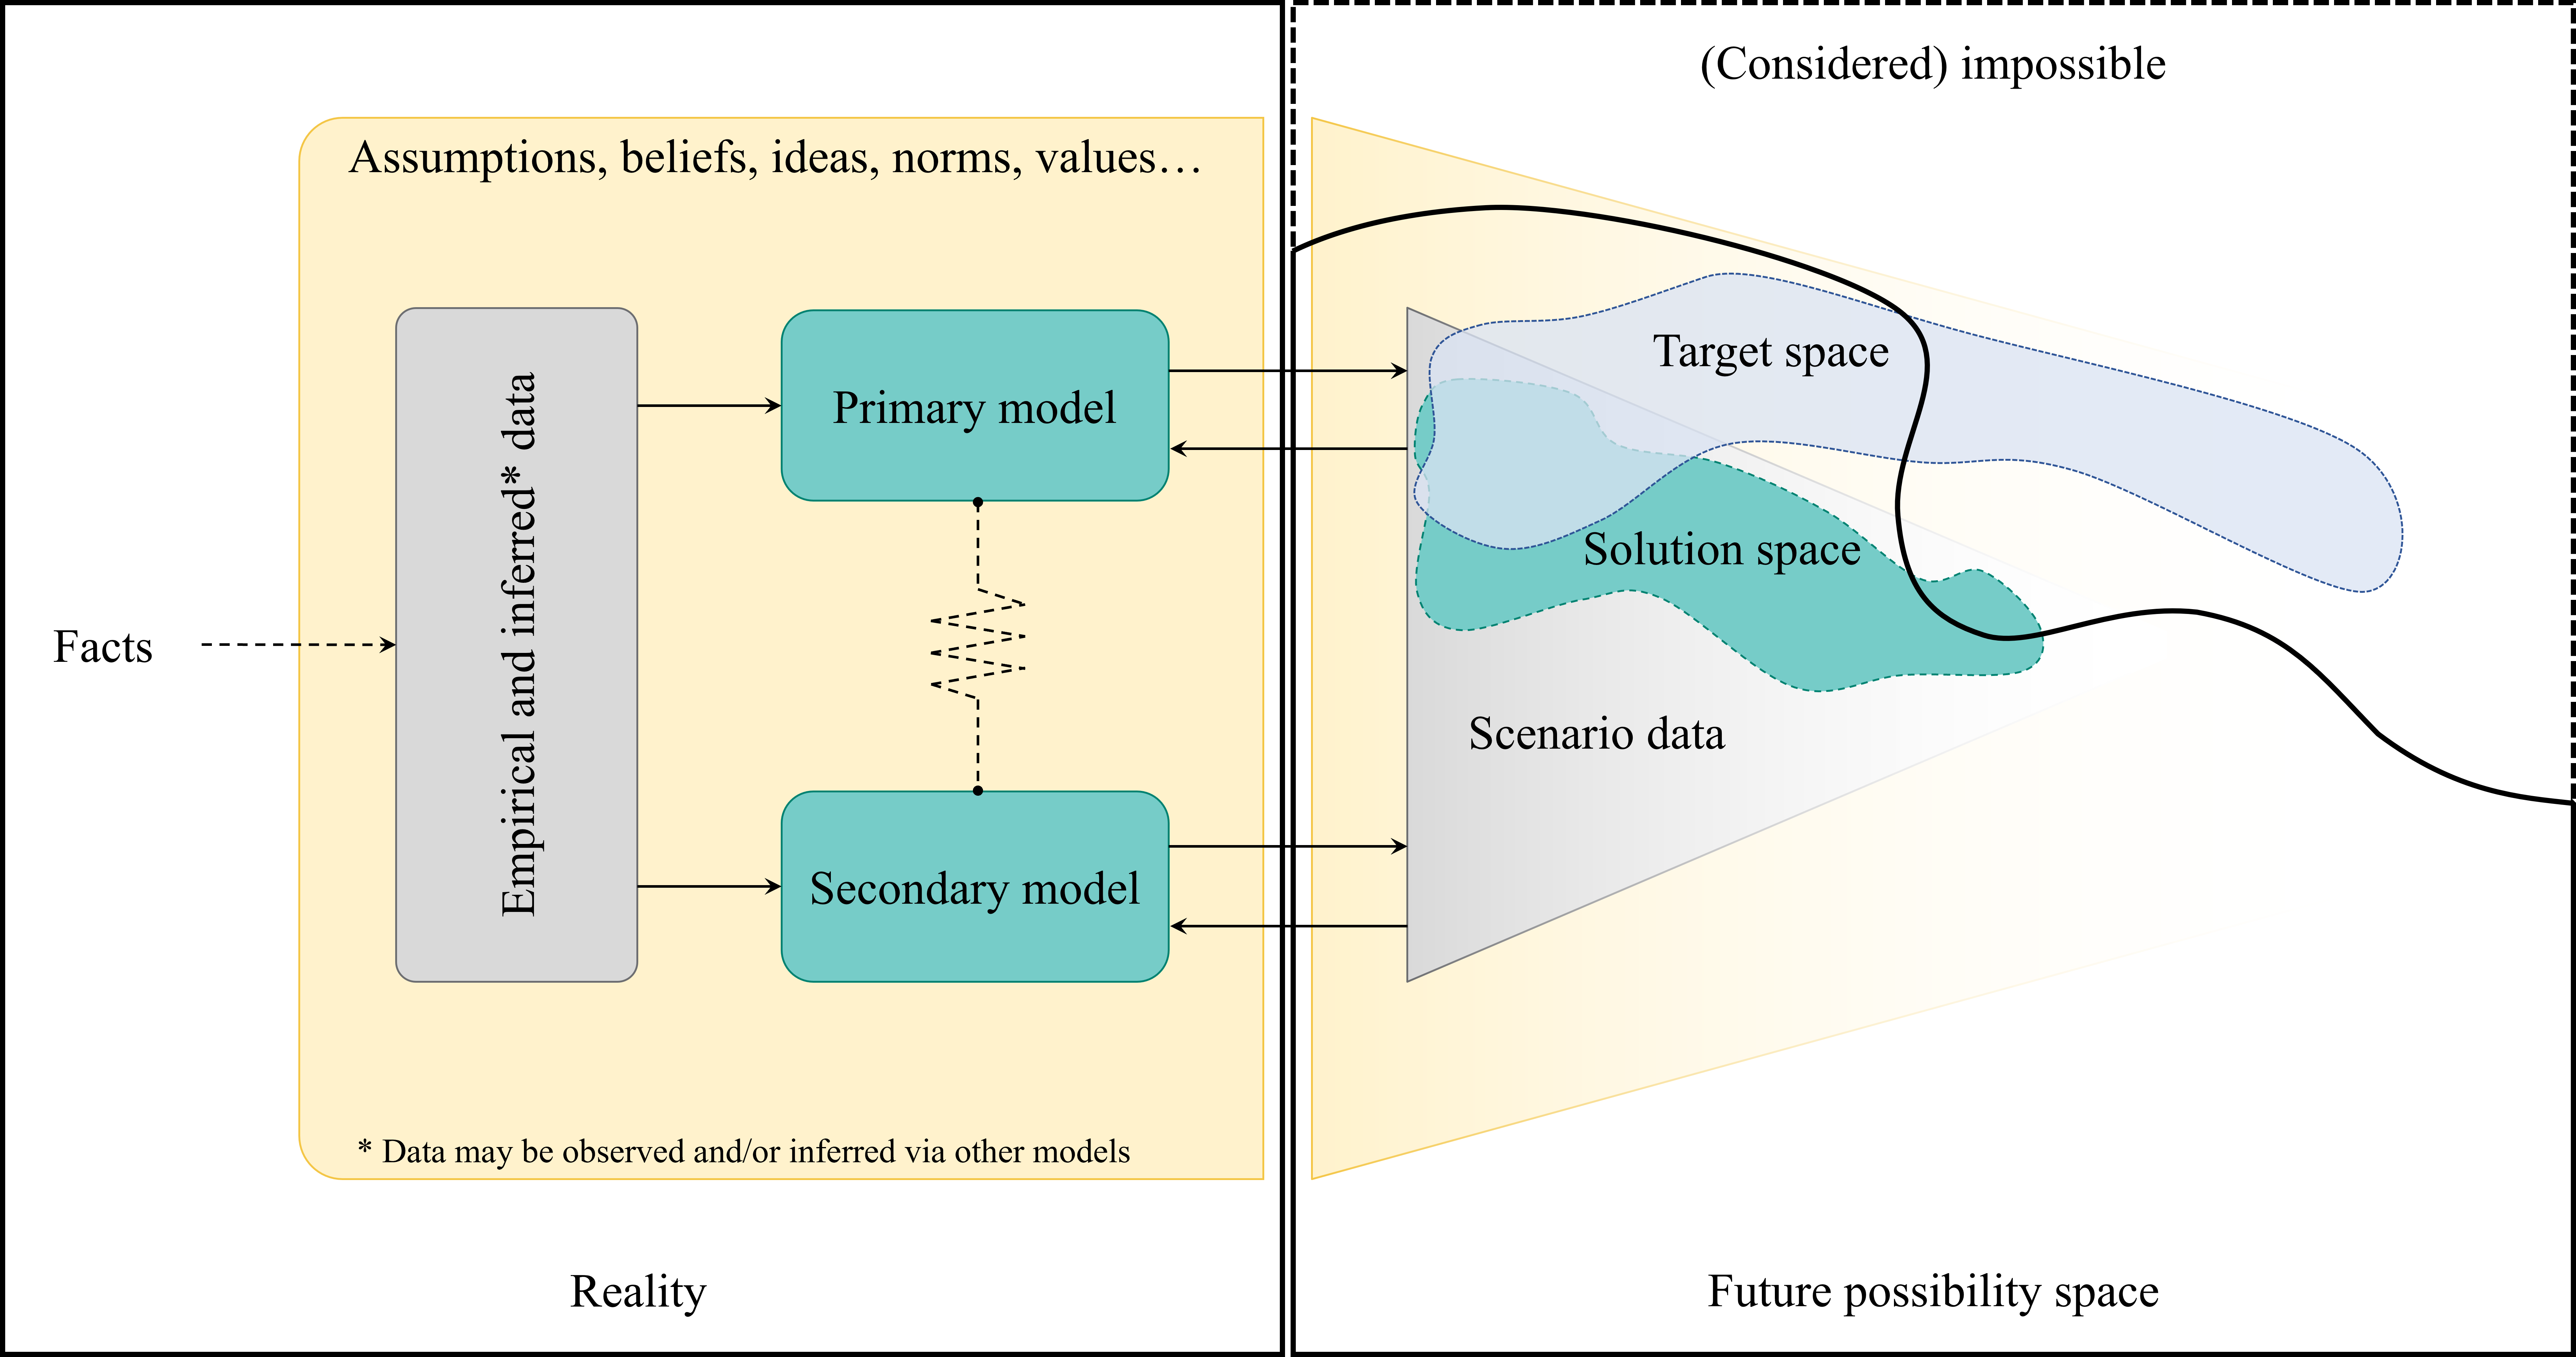
\includegraphics[width=\textwidth]{Model_spaces.png} 
    \caption[Another caption for list of figures]{Models use and produce data and may influence each other. The future consists of different spaces, which may differ dependent on which model is used.}
    \label{fig:model_spaces}
\end{figure}


\label{main_part}
\section{Positionality, reflexivity, and interdependency}

Basically reiterate many of the points made by Lazurko et al. but apply to the present case, i.e. when models inform each other (via coupling or not)

Add my points on primary and secondary models. Supported by figure 2. 
Primary models being primarily IAMs, and secondary models for example IE models. Another way of seeing it is that primary models are causal/dynamic models, and secondary models are attributional models. Or: primary models are those with which authoritative scenario sets are created, and secondary models are those which use (adapt/customise) these scenarios then.

Idea behind figure: 
Reality provides facts. 
Facts are observed (therefore data) and shape our assumptions beliefs, norms etc. 
Our assumptions etc. determine in turn which data we collect. 
Existing data are used as inputs for primary and secondary models. 
These models can be coupled, either hard or soft - or not at all. 
--
We also have assumptions etc about the future. 
These assumptions etc. form, however, only a subspace of the full possibility space. 
At the same time, our assumptions etc. shape the possibility space. 
Primary and secondary models may be used for scenario modelling, generating and potentially also using scenario data. 
Scenario data consists of exogenous and endogenous halves. The exogenous part is determined by our assumptions etc. about the future whereas endogenous part is determined through the model (which is based on past/current data and/or assumptions etc.). 
Often, scenario data generated with primary models is used for further analysis with secondary models, with conflicts of assumptions and ambiguities being a possible result. 
The solution space contains those parts of the scenario data which were/could be computed for a given single scenario. 
Target space describes what is desirable in terms of targets. 
We might have some targets that lie outside of what can be examined with the models (target space outside of solution space). 
Some targets may be impossible, e.g. because various targets are conflicting. 
We have assumptions about what the future could be like, but that future might simply not be possible.

Our exploration regards in particular the cases when the interaction between primary and secondary models is of a soft-coupled or selective-data-adoption nature, which may often be the case when existing large-scale (e.g. global) scenario sets are downscaled.

"either the process of developing the scenarios can be connected or the elements and outcomes of the scenarios can be linked (Zurek and Henrichs 2007)" in Biggs et al. \url{https://www.ecologyandsociety.org/vol12/iss1/art17/}; Zurek and Henrichs \url{https://doi.org/10.1016/j.techfore.2006.11.005}

Adapting and customising scenarios with secondary models naturally leads to continuing someone else's model-land (\url{https://www.degruyter.com/document/doi/10.5018/economics-ejournal.ja.2019-40/html}), a situation in which reflexivity practice (Luzarko et al.) can help reduce ambiguities and inconsistencies. (Some ambiguities and inconsistencies might remain, e.g. some assumptions remaining hidden no matter what as McDowall and Geels pointed out \url{https://doi.org/10.1016/j.eist.2016.07.001})

Someone's plausible scenario output might be someone else's implausible scenario input (and vice versa)


\section{Moving forward}

Recap + recommendation + conclusion

\begin{itemize}
    \item provide guidance on how reflexivity practice could be adopted by secondary modellers. At least, the use of scenario qualifiers needs to be adopted.
    \item secondary modelling should explore the existing possibility space more comprehensively (e.g. by not only taking SSP marker scenarios as inputs).
    \item extreme events need to be explored more comprehensively. Perhaps include "dummy extreme events", i.e. possible disruptions of some parameters along the way (at some time step), perhaps even "compund extreme events" (which may push the actual pathway far from what is currently considered plausible). Similarly, create perhaps a "very worst case" scenario where all such possible disruptions happen (applied to all parameters)
    \item for both primary and secondary modelling: reduce sectoral (+spatiotemporal) resolution when further in the future
\end{itemize}

\newrefcontext[sorting=nyt] % sort the paper by name, year, title
\printbibliography[heading = bibintoc] % 'bibintoc' inserts our bibliography into the table of contents

\end{refsection}

%%%%%%%%%%%%%%%
%% Appendix
%% Inserting appendix with separate settings
%\newpage
%\setcounter{page}{1}
%\renewcommand{\thepage}{A-\arabic{page}}
%\linenumbers*
%\addappendix
%
%%Reset numbering of tables and equations in appendix, starting with A.
%\renewcommand{\thetable}{A.\arabic{table}}
%\setcounter{table}{0}
%\renewcommand{\theequation}{A.\arabic{equation}}
%\setcounter{equation}{0}
%
%\begin{refsection}
%\section*{Appendix A}
%BLABLA
%
%\section*{Appendix B}
%blabla
%
%\nolinenumbers
%\newpage
%\newrefcontext[sorting=nyt] % sort the paper by name, year, title
%\printbibliography[title = References in appendix]
%
%\end{refsection}
\end{document}